\documentclass[twoside]{article}
\setlength{\oddsidemargin}{0.25 in}
\setlength{\evensidemargin}{-0.25 in}
\setlength{\topmargin}{-0.6 in}
\setlength{\textwidth}{6.5 in}
\setlength{\textheight}{8.5 in}
\setlength{\headsep}{0.75 in}
\setlength{\parindent}{0 in}
\setlength{\parskip}{0.1 in}

\usepackage{graphicx}
\usepackage{url}
\usepackage{listings}
%
% The following commands sets up the lecnum (lecture number)
% counter and make various numbering schemes work relative
% to the lecture number.
%
\newcounter{lecnum}
\renewcommand{\thepage}{\thelecnum-\arabic{page}}
\renewcommand{\thesection}{\thelecnum.\arabic{section}}
\renewcommand{\theequation}{\thelecnum.\arabic{equation}}
\renewcommand{\thefigure}{\thelecnum.\arabic{figure}}
\renewcommand{\thetable}{\thelecnum.\arabic{table}}
\newcommand{\dnl}{\mbox{}\par}

%
% The following macro is used to generate the header.
%
\newcommand{\lecture}[4]{
  \pagestyle{myheadings}
  \thispagestyle{plain}
  \newpage
  \setcounter{lecnum}{#1}
  \setcounter{page}{1}
  \noindent
  \begin{center}
  \framebox{
     \vbox{\vspace{2mm}
   \hbox to 6.28in { {\bf CMPSCI~630~~~ Systems
                       \hfill Spring 2017} }
      \vspace{4mm}
      \hbox to 6.28in { {\Large \hfill Lecture #1  \hfill} }
%       \hbox to 6.28in { {\Large \hfill Lecture #1: #2  \hfill} }
      \vspace{2mm}
      \hbox to 6.28in { {\it Lecturer: #3 \hfill Scribe: #4} }
     \vspace{2mm}}
  }
  \end{center}
  \markboth{Lecture #1: #2}{Lecture #1: #2}
  \vspace*{4mm}
}

%
% Convention for citations is authors' initials followed by the year.
% For example, to cite a paper by Leighton and Maggs you would type
% \cite{LM89}, and to cite a paper by Strassen you would type \cite{S69}.
% (To avoid bibliography problems, for now we redefine the \cite command.)
%
\renewcommand{\cite}[1]{[#1]}

% \input{epsf}

%Use this command for a figure; it puts a figure in wherever you want it.
%usage: \fig{NUMBER}{FIGURE-SIZE}{CAPTION}{FILENAME}
\newcommand{\fig}[4]{
           \vspace{0.2 in}
           \setlength{\epsfxsize}{#2}
           \centerline{\epsfbox{#4}}
           \begin{center}
           Figure \thelecnum.#1:~#3
           \end{center}
   }

% Use these for theorems, lemmas, proofs, etc.
\newtheorem{theorem}{Theorem}[lecnum]
\newtheorem{lemma}[theorem]{Lemma}
\newtheorem{proposition}[theorem]{Proposition}
\newtheorem{claim}[theorem]{Claim}
\newtheorem{corollary}[theorem]{Corollary}
\newtheorem{definition}[theorem]{Definition}
\newenvironment{proof}{{\bf Proof:}}{\hfill\rule{2mm}{2mm}}

% Some useful equation alignment commands, borrowed from TeX
\makeatletter
\def\eqalign#1{\,\vcenter{\openup\jot\m@th
 \ialign{\strut\hfil$\displaystyle{##}$&$\displaystyle{{}##}$\hfil
     \crcr#1\crcr}}\,}
\def\eqalignno#1{\displ@y \tabskip\@centering
 \halign to\displaywidth{\hfil$\displaystyle{##}$\tabskip\z@skip
   &$\displaystyle{{}##}$\hfil\tabskip\@centering
   &\llap{$##$}\tabskip\z@skip\crcr
   #1\crcr}}
\def\leqalignno#1{\displ@y \tabskip\@centering
 \halign to\displaywidth{\hfil$\displaystyle{##}$\tabskip\z@skip
   &$\displaystyle{{}##}$\hfil\tabskip\@centering
   &\kern-\displaywidth\rlap{$##$}\tabskip\displaywidth\crcr
   #1\crcr}}
\makeatother

% **** IF YOU WANT TO DEFINE ADDITIONAL MACROS FOR YOURSELF, PUT THEM HERE:



% Some general latex examples and examples making use of the
% macros follow.

\begin{document}

%FILL IN THE RIGHT INFO.
%\lecture{**LECTURE-NUMBER**}{**DATE**}{**LECTURER**}{**SCRIBE**}
\lecture{17}{April 14}{Emery Berger}{Jayanth Parameshwar Hegde,Daniel Sam Pete Thiyagu}

\section*{GProf}

Terminology:

Static call graph: Generated using static analysis. This graph depicts all possible function calls in an execution of the program and the arrows indicate the flow of control.

Consider the following program snippet:

\begin{lstlisting}[language=C]
void foo(){
    a();
    b();
}

void bar(int n){
    if(n!=0){
        c();
        a();
        bar(n-1);
    }
}

int main(){
    foo();
    bar(10);
    return 0;
}

\end{lstlisting}

Static call graph for the above program:

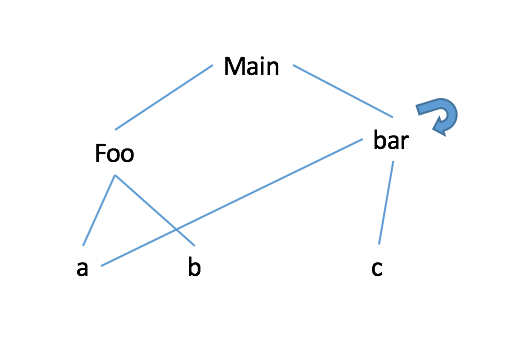
\includegraphics[scale=0.5]{static_call_graph}

Dynamic call graph: Generated from an execution of the program. Nodes represent only the function calls 
observed during this particular execution and the arrows indicate  the flow of control. The profiling is more detailed.

Dynamic call graph \subseteq static call graph

Probe effect: Distortion in measurement due to the act of measuring.
Example: In order to profile a function, one might copy all parameters to a storage. When the size of parameters
is large or the number of parameters is large, this copying might evict lot of information of caches. This leads
to cache misses worsening the performance of the program under profiling.

Solution to probe effect: Arnold-Ryder approach (based on sampling)
The program counter values are sampled at regular intervals of time. Using the distribution of these sampled values, execution times are inferred. This mitigates probe effect and cost of profiling.

Problems with sampling: Applications with heartbeat messages or alternate busy and idle intervals can lead to wrong profiling. The idle times may coincide with the sampling time and cause the profiler to capture nothing. This is solved using Nyquist's theorem where you should always sample double the frequency. 


Perf is a Unix profiling tool based on sampling. 
\textbf{Perf Tool}
It is an on-chip ARM counter and can count cache misses at every level, branch mispredictions, instructions retired. It records the call stack. 

For example let us consider call stacks like 

main() \(->\) foo() \(->\) a()

main() \(->\) foo() \(->\) b()

the sequence of calls are that a is called first and b is called 99 times , and a is then called again once and b is called 99 times again and so on. Say if we have the countdown timer that checks every 100 times, then our profiler would say that a is the most frequently called code and you would need to optimize the function a , whereas the function b is the most frequently called. Only if it is uniformly distributed, this(countdown timer approach) works well. So sampling should be random.



Gprof profiling:

Gprof produces flat profiles. A flat profile makes measurements of a function execution independent of the
callee. Thus, it is path/context insensitive. Alternatively a path sensitive profiling breaks down measurements
with respect to the path taken. Depending on the path taken in a particular execution, the measurements can
vary. Also flat profiling looks at every function independently and it doesn't account for hierarchy.



Some other notes: 
\begin{itemize}
    \item Gprof cant profile multi-threaded code
    \item Probe effect is seen with Gprof
    \item The calls that arise to the kernel space from the user space is not profiled.
    \item Sampling based profilers were state of the art before coz.
    \item In multithreaded profilers, we have critical path, longest path. Making improvements on the critical path may not be worth doing if improvements dont reflect in increase in performance.
    
    
\end{itemize}





\section*{Notes on stabilizer, randomizations}
This was a continuation of some of the topics discussed in the previous lecture.

Experimental Setup Randomization :

Let us consider link object ordering, and say there are 4 object files and we have 4! possible orderings and a program like google chrome has around 10000 object files and it is impossible to do such testing. So experimental setup randomization helps us to get an approximation based on average sampling. 

Randomization hurts locality. The objects wont be stored contiguously. But inside an object/page, locality wont be impacted. The overhead of stabilizer arises from the fact that TLB(mapping from virtual to physical pages) is impacted and TLB misses are costly and degrades performance.

\section*{Byzantine Problem}
The need for Distributed systems started with the creation of the World Wide Web in 1993

In an asynchronous distributed consensus system, there are no leaders and everyone is equal.

For distinguishing between message failure and delay we need to have a bounded delay and this can also involve getting repeated messages. Things can fail and there could be traitors who could also decide to be evil. The most possible general failure model includes forging messages. If there are m number of malicious actors and 3m+1 loyal good guys then it is impossible to forge messages. In general you dont know the number of malicious users.
Byzantine generals is used for security and reliability.



\textbf{Byzantine Fault Tolerance}
Handling independent random faults



\end{document}
